
%%%%%%%%%%%%%%%%%%%%%%% file typeinst.tex %%%%%%%%%%%%%%%%%%%%%%%%%
%
% This is the LaTeX source for the TDPTemplate using
% the LaTeX document class 'llncs.cls' Springer LNAI format
% used in the RoboCup Symposium submissions.
% http://www.springer.com/computer/lncs?SGWID=0-164-6-793341-0
%
% It may be used as a template for your own TDP - copy it
% to a new file with a new name and use it as the basis
% for your Team Description Paper
%
% NB: the document class 'llncs' has its own and detailed documentation, see
% ftp://ftp.springer.de/data/pubftp/pub/tex/latex/llncs/latex2e/llncsdoc.pdf
%
%%%%%%%%%%%%%%%%%%%%%%%%%%%%%%%%%%%%%%%%%%%%%%%%%%%%%%%%%%%%%%%%%%%

\documentclass[runningheads,a4paper]{llncs}
\usepackage{amssymb}
\setcounter{tocdepth}{3}
\usepackage{graphicx}
\usepackage{amssymb}
\usepackage[utf8]{inputenc}
\usepackage{url}
\usepackage{float}
\usepackage{amsmath}
\usepackage{graphicx}
\usepackage{wrapfig}
\usepackage{tabto}
\usepackage{lipsum}
\usepackage[table,xcdraw]{xcolor}
\usepackage{hyperref}
\usepackage{subcaption}

\newcommand\notes[1]{\textcolor{red}{#1}}


\begin{document}


\newif\ifdraft
\draftfalse


\ifdraft
\setlength{\belowcaptionskip}{-5pt}
\fi

\title{Walking Machine @Home \newline \: 2019 Team Description Paper}

\author{Jeffrey Cousineau, Huynh-Anh Le, et al.}
\institute{École de Technologie Supérieure \\ 1100 rue Notre-Dame Ouest, Montreal, QC, Canada H3C 1K3 \\
\texttt{http://walkingmachine.ca,} \texttt{walking@ens.etsmtl.ca,} \texttt{https://github.com/WalkingMachine}}
\maketitle


%%%%%%%%%%%%%%%%%%%%%%%%%%%%%%%%%%%%%%%%%%%%%%%%%%%%%%%%%%%%%%%%%%%%%%%%%%%%%%%%%%%%

\begin{abstract}

This paper gives details about the RoboCup@Home league team Walking Machine, from ETS University in Montreal, Canada for the next competition in Sydney, in July 2019. The robot from Walking Machine, named S.A.R.A. for "Systeme d'Assistance Robotique Autonome" (in English, Automated Robotic Assistance System), is a robot entirely built by the scientific club from ETS, mainly composed of undergraduates students. The robot is used for social interaction with humans, navigation and object manipulation. This document shows the electrical, mechanical and software novelties and functionalities of S.A.R.A.

\end{abstract}

%%%%%%%%%%%%%%%%%%%%%%%%%%%%%%%%%%%%%%%%%%%%%%%%%%%%%%%%%%%%%%%%%%%%%%%%%%%%%%%%%%%%

\section{Introduction}
\tab Walking Machine’s team is a young team from Montreal, Quebec, in Canada, composed of engineering students in the field of mechanical, electrical and software engineering. We have been working really hard to improve our robot for the next year Robocup@Home competition. As this would be our fourth participation, we learned a lot at Montreal Robocup and we made many improvements to get better results, mostly on the software side. In the past, the team went in many competitions like the Eurobot, but made the leap for the RoboCup@Home competition to get a bigger challenge and to get an opportunity to bring novelty in the scientific community surrounding robotic. \\


SARA, our creation, was designed for polyvalent human-robot interaction as well as efficient navigation and object manipulation. Our robot is mounted on four mecanum wheels powered by Roboteq drives, has one arm mimicking a normal human arm, and sensors for communication and navigation. Our team has developed knowledge in object and people detection/recognition, as well as navigation using a laser scanner, odometry on the wheels and a Asus Xtion camera. All of these parts are interfaced through ROS (Robot Operating System). \\

\section{Mechanical improvement}

\subsection{Mechanical}

\tab To improve our robot habilities, we decide to add a vertical linear actuator, more specifically, a TL5 column made by TiMOTION. This will add a degree of freedom, giving us a wider range of motion to reach objects on the floor or higher on the cupboard shelves. This will be really helpful for challenge like storing groceries where the objects can be anywhere in the cupboard. \\

\begin{figure}[h!]
  \centering
  \begin{subfigure}[b]{0.2\linewidth}
    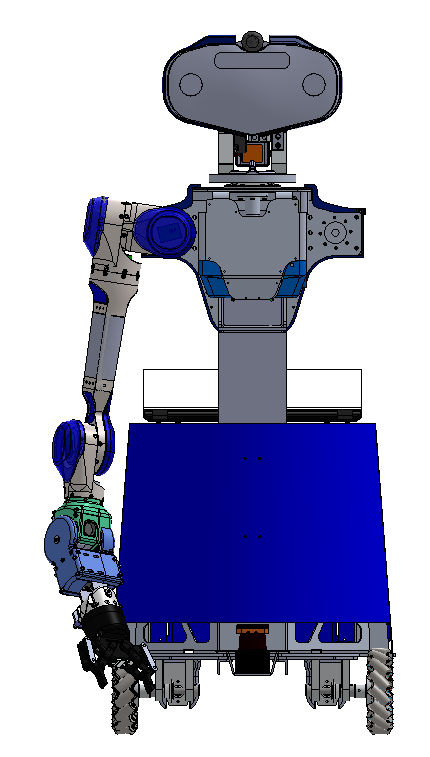
\includegraphics[width=\linewidth]{images/robot_low.PNG}
    \caption{Lowest point}
  \end{subfigure}
  \begin{subfigure}[b]{0.2\linewidth}
    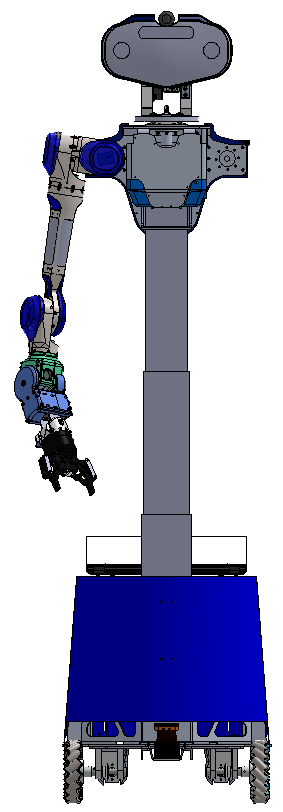
\includegraphics[width=\linewidth]{images/robot_high.PNG}
    \caption{Highest point}
  \end{subfigure}
  \caption{S.A.R.A. linear actuator motion range}
  \label{fig:coffee}
\end{figure}

We also decided to improve our wrist by adding a gearbox, giving it more strength. We took the decision to improve it after having problems with the gripper being too heavy.  

\newpage
\section{Software}

\subsection{High-level task planning}
\tab For our task planning, we use a state machine software developed by team Vigir, one of the participants of the Darpa Robotics Challenge. This software, named \href{http://philserver.bplaced.net/fbe/index.php}{FlexBe}\cite{schillinger2016flexbe}, for Flexible Behavior, is a block-based interface for making state machines.\\

\begin{figure}[h!]
	\centering
	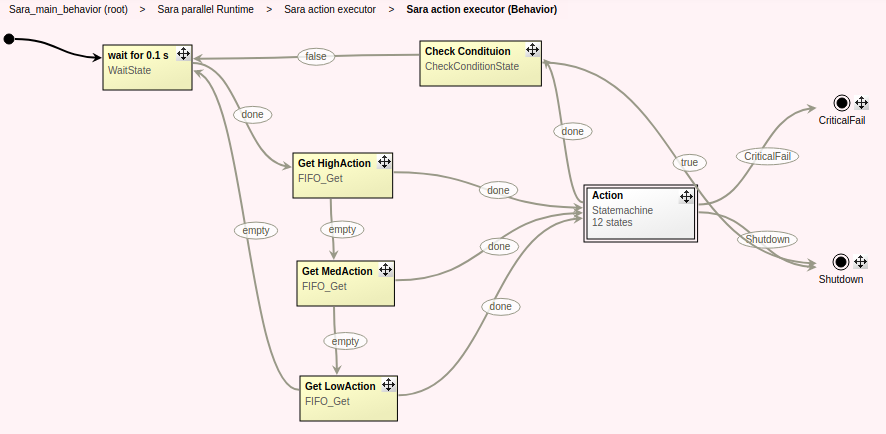
\includegraphics[width=0.70\textwidth]{images/flexbe.png}
	\caption{FlexBe behavior representation}
\end{figure}

But we do not simply use FlexBe as is. We still need to write our own states using its python API. To simplify our work, we started by splitting all of the Robocup@home scenarios into basic actions. We then identified all of these basic actions our platform could accomplish and we confined them in blocks named States, e.g. MoveArm, MoveHead etc. These blocks can then be assembled together to form a higher level of blocks we named Actions e.g. Pick, LookAt etc. Those Actions can then again be assembled into what we call ActionWrappers. The role of ActionWrapper is to allow interfacing our Actions with our natural language processing software(see natural language processing below). They receive the segmented text and translate it to computer understandable parameters using our Wonderland (see environment reasoning below) knowledge base and other sources of information. This recursive structure allows us to quickly develop our robot’s behaviours.\\

\subsection{Natural language processing}
\tab 


\subsection{Object recognition}
\tab For our object recognition, we use YOLO \cite{yolo}, a real-time object detection. It does not only detect various object but it also predicts the bounding boxes of the detected object. It uses a single neural network which is applied to the image. Multiple regions are then created and are used to predict the bounding boxes. Each of them also contains the predicted probability which is used to filter the predicted objects. The advantage of this system is that it can detect multiple objects in a real-time scenario.\\
 
\begin{figure}
  \centering
  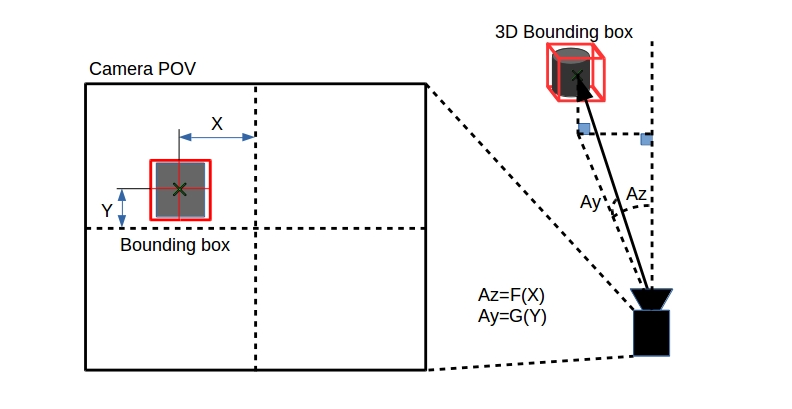
\includegraphics[width=200pt]{images/frame_to_box.png}
  \caption{2D bounding box to 3D grasping pose, current technique}
\end{figure} 
 


\begin{figure}
  \centering
  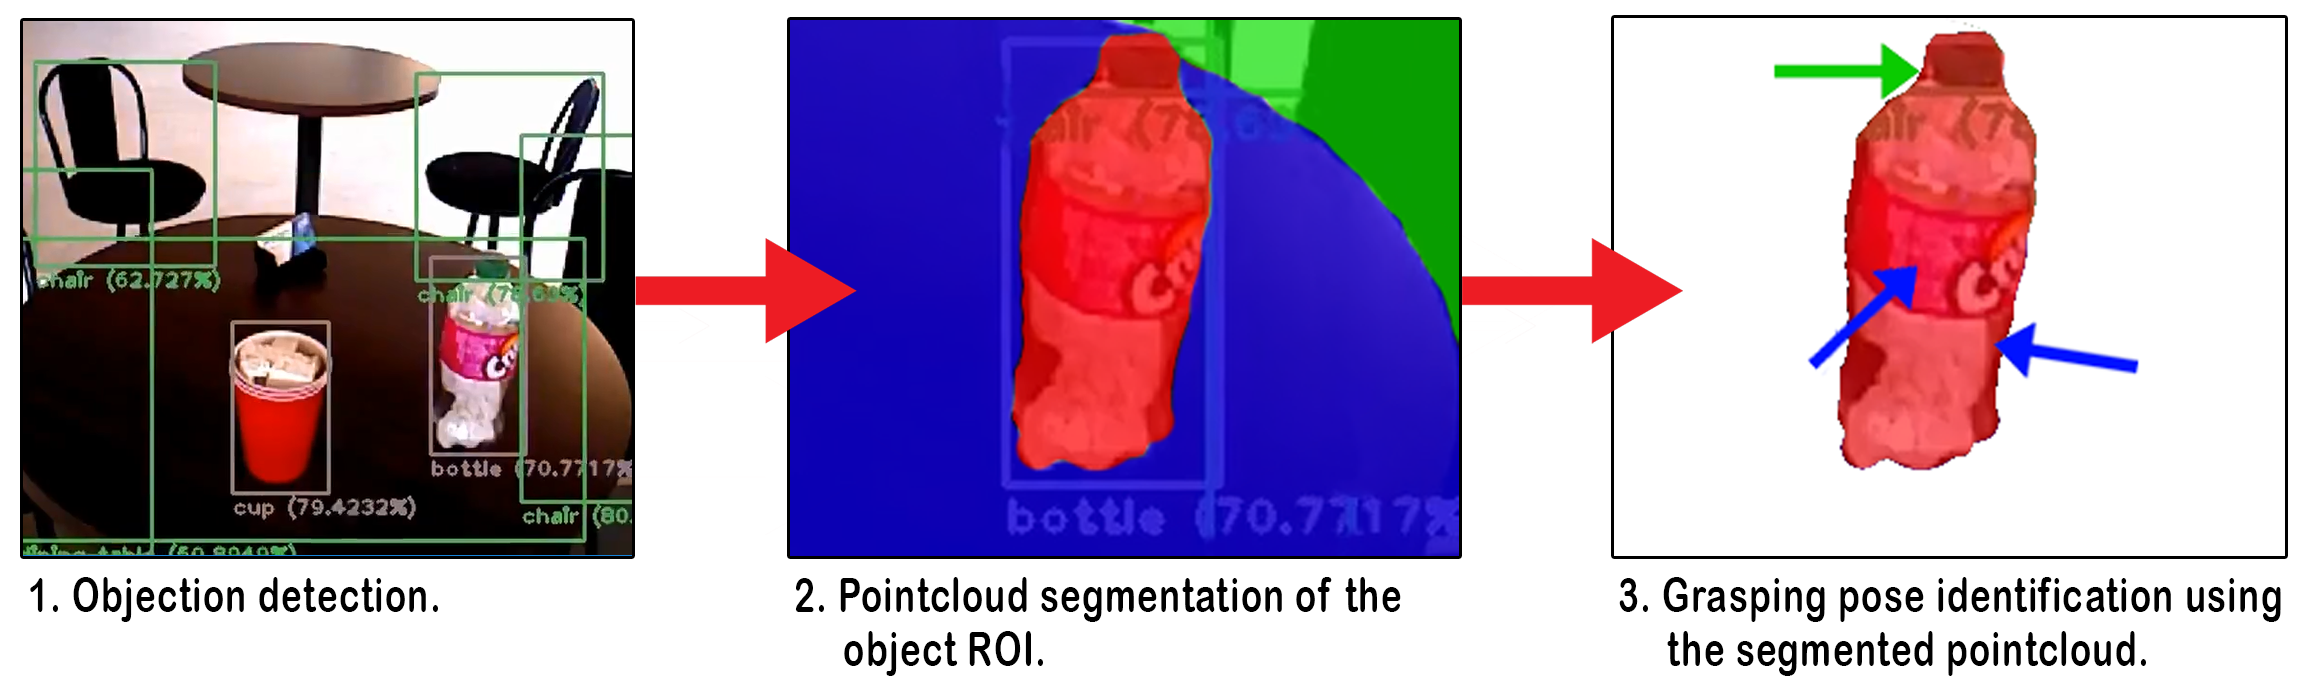
\includegraphics[width=300pt]{images/frame_to_box2.png}
  \caption{2D bounding box to 3D grasping pose, future technique}
\end{figure}

For the moment, we are using the YOLO model but, we are looking forward to training our own dataset, just like we would do in competition. This is new for us but we have all the tools we need to overcome this. \\

\subsection{Navigation}
\tab In addition to last year navigation stack, this year we are using the \href{http://wiki.ros.org/pointcloud_to_laserscan}{pointcloud\_to\_lasercan} package as a lighter solution for 3D mapping and obstacle avoidance. This ensures a safe navigation around objects like table or chair since only the legs are detected by the lidar laser. Another great thing about this implementation is the fact that we can set the maximum height for collision avoidance. That way, if there’s an obstacle at head level, our robot will avoid it the same way it would with an object on the floor. \\

\subsection{Environmental reasoning}
\tab As a novelty this year, we implemented our own solution for an environment representation in a way that we think is simple and easy for everyone. Our package named \href{http://github.com/walkingmachine/wonderland}{wonderland} is an agnostic system in the same way than LU4R. It’s composed of a server that received HTTP query based on a custom API. \\

The first thing that is needed when you start using this platform is to populate the database. This can be done manually if you already know the object position, but this can be done by your robot through POST query. It’s also possible to specify some room with a specific position relates to it. Once this is done, you can call our API and for example, just by doing a GET request on the URL http://wonderland:8000/object, this will return you the list of every object the database contains. It’s also possible to filter the request by giving a known color, link to the object or a location as a parameter. \\

Since the database is hosted as a server, you can access it from everywhere. You could decide to export it to another computer, run it in the cloud or just put it on the robot system itself. It also gives the possibility to have a dynamic knowledge, meaning that the robot can update its knowledge of his environment in real-time. \\



\section{Conclusions and future work} 
\notes{Pourrait être rephrasé.}
As you can see, despite being a group of undergraduate students, our team is about to catch up with the rest of the league. We’ve recently put a lot of efforts into stabilizing our platform and fixing as many bugs as possible to give us a strong foot to move forward.\\

\notes{Actualiser le dernier paragraphe.}
With its new swappable batteries system, object detection network and natural language processing, our robot has become a fully functional autonomous platform allowing us to focus our efforts on the challenges themselves instead of continuously fixing our hardware.
\\

\section*{Robot SARA Hardware Description}
% TODO Change picture and description
Specifications for robot SARA are as follows:

\begin{table}

\label{my-label}

\begin{tabular}{l|p{90mm}}
\hline
\rowcolor[HTML]{FFFFFF} 
\multicolumn{2}{c}{\cellcolor[HTML]{FFFFFF}\textbf{SARA}}                                                      \\ \hline
\rowcolor[HTML]{EAEFF6} 
\textbf{Base}               & Custom base with fully holonomic platform                                        \\
\rowcolor[HTML]{FFFFFF} 
\textbf{Right arm}          & 7 DoF custom arm made of Kinova motors                                           \\
\rowcolor[HTML]{EAEFF6} 
\textbf{Neck}               & Tilt and pan unit using two Dynamixel MX-64R servo actuator                      \\
\rowcolor[HTML]{FFFFFF} 
\textbf{Head}               & Custom head made of RGB neopixels leds and Asus Xtion Pro                        \\
\rowcolor[HTML]{EAEFF6} 
\textbf{Gripper}            & Robotiq 2 fingers 140mm                                                           \\
\rowcolor[HTML]{FFFFFF}
\textbf{Dimensions}         & \begin{tabular}[c]{@{}l@{}}Base : 0,61m. X 0,77m.\\ Height : 1,68m.\end{tabular} \\
\rowcolor[HTML]{EAEFF6} 
\textbf{Weight}             & $\sim$60kg                                                                      \\
\rowcolor[HTML]{FFFFFF} 
\textbf{Additional sensors} & Hokuyo UTM-30LX on base                                                          \\
\rowcolor[HTML]{EAEFF6} 
\textbf{Microphone}         & Rode microphone											                         \\
\rowcolor[HTML]{FFFFFF} 
\textbf{Batteries}          & 2x 20V Dewalt drill battery 5aH                                                 \\
\rowcolor[HTML]{EAEFF6} 
\textbf{Computer}           & 1x Lenovo p50 with 32GB RAM and nVidia Quadro M2000 4GB, 1x Raspberry Pi 3       \\ \hline
\end{tabular}
\caption{Robot's hardware description}
\end{table}
\begin{wrapfigure}[10]{r}{0.25\textwidth}
	\centering
	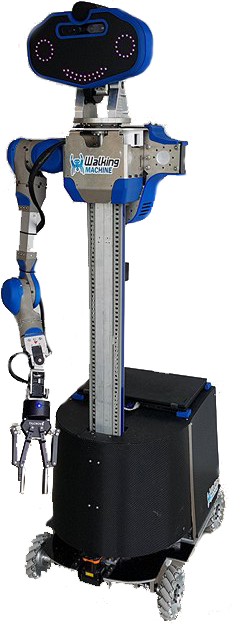
\includegraphics[width=0.30\textwidth]{images/sara_2.png}
	\caption{Robot SARA}
\end{wrapfigure}
\section*{Robot's Software Description}

For our robot we are using the following software:

\begin{itemize}
	\item Platform: Robotic Operating System (ROS) Kinetic on Ubuntu 16.04
	\item Navigation, localization and mapping: \href{http://wiki.ros.org/gmapping}{Gmapping}, \href{http://wiki.ros.org/amcl}{AMCL}, \href{http://wiki.ros.org/pointcloud_to_laserscan}{pointcloud\_to\_laserscan}
	\item Face recognition: \href{http://wiki.ros.org/people}{People}
	\item Speech recognition: \href{https://github.com/WalkingMachine/lab_ros_speech_to_text}{Google Speech API}
	\item Speech comprehension: \href{http://sag.art.uniroma2.it/lu4r.html}{LU4R}, \href{https://github.com/WalkingMachine/lu4r_ros}{lu4r\_ros}
	\item Speech generation: \href{https://doc.ubuntu-fr.org/svoxpico}{Svoxpico}
	\item Object recognition: \href{https://github.com/WalkingMachine/wm_darknet}{Darknet with YOLO v2 }
	\item Arm control: \href{http://wiki.ros.org/moveit}{MoveIt} and \href{https://github.com/Kinovarobotics/kinova-ros}{Kinova API}
	\item Task executor: \href{http://wiki.ros.org/flexbe}{Flexbe} 
	\item World reprensentation: \href{http://github.com/walkingmachine/wonderland}{Wonderland}
\end{itemize}
	
\section*{Team members}
André-Philippe Audette,
Nicolas Bernatchez,
Pierre-Emmanuel Billeau,
Jeffrey Cousineau, 
Raphael Duchaine,
Quentin Gaillot,
Louis-Charle Labarre, 
Philippe La Madeleine,  
Redouane Laref,
Vincent Lavoie-Marchildon,
Huynh-Anh Le,
Lucas Maurice,
Alexandre Mongrain,
Jimmy Poirier,
Veronica Romero Rosales

\nocite{*}
\bibliographystyle{plain}
\bibliography{references}


\end{document} 
